\section{Работа с имитационной моделью}
В данном разделе изложены подходы к работе с реализованным пакетом программ, показывающие течение процесса исследования при помощи имитационного моделирования и дополнительных утилит для расчета характеристик. 
\subsection{Определение области применимости асимптотических результатов исследования модели RQ--системы с повторными вызовами и обратной связью}

В главе \ref{rq_3} описаны асимптотические результаты, в частности приближение характеристической функции числа обслуженных заявок разного типа за время $t$. Последующей задачей ставится определение области применимости полученного приближения. 

\begin{figure}[H]
	\centering
	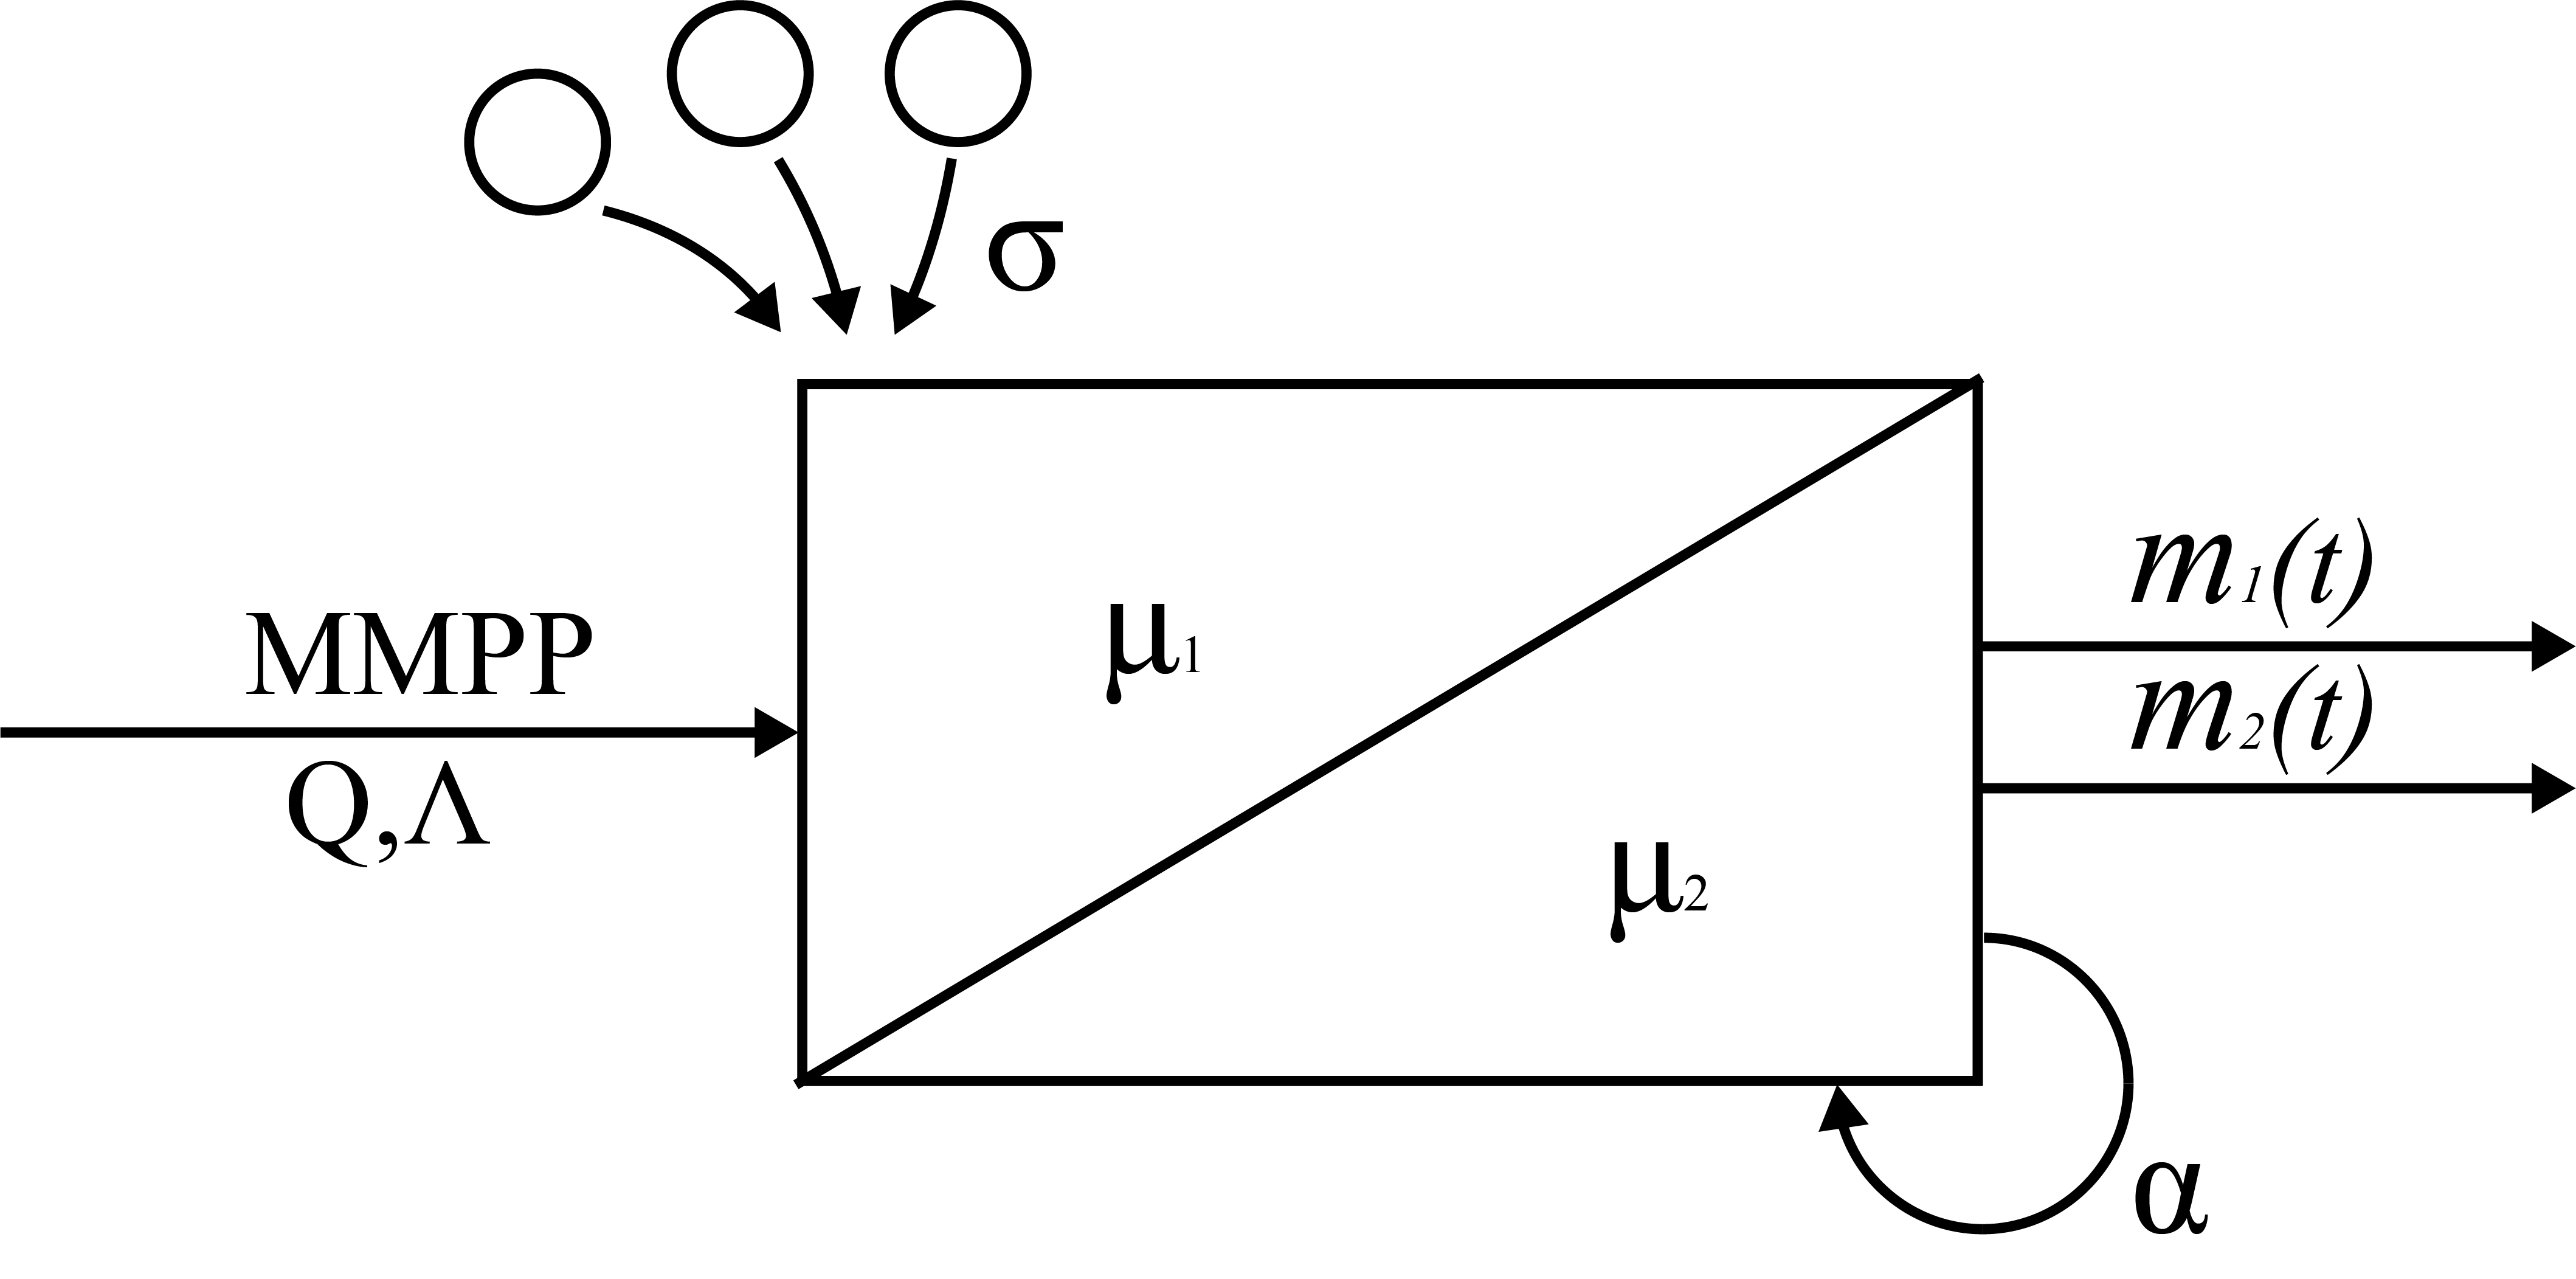
\includegraphics[scale=0.4]{RQ.png}
	\caption{Модель RQ--системы с повторными вызовами и обратной связью} \label{rq_system}
\end{figure}

Поскольку решение было получено при асимптотическом условии бесконечной задержки заявок в источнике повторных вызовов, требуется определить, при каких параметрах модели асимптотические результаты становятся недостоверными. Для это цели как раз отлично подходит имитационное моделирование.

В первую очередь, импортируем модуль наш q\_analysis. Он, в свою очередь, содержит подмодуль simulation для имитационного моделирования. Именно содержит реализацию ранее описанной предметной области.
\begin{pyin}
	import q_analysis.simulation as q
\end{pyin}
Создадим модель и установим время моделирования, равное 1000000 условных единиц.
\begin{pyin} 
model = rq.Model()
model.set_time(0) 
model.set_end(100000)
model
\end{pyin}

\begin{pyout}
	Model{ time: 0, end : 1000000, event_queue_len : 0, num_components : 0, num_connections : 0 }
\end{pyout}

Далее добавим элементы модели (метод add\_producer). 

В модель добавятся следующие элементы: 
\begin{itemize}
	\item MMPP поток c матрицей $\Lambda$ следующего вида
		\begin{equation*}
			\Lambda =  \begin{bmatrix}
			1.0 & 0 &  0\\
			0 & 1.12 & 0\\
			0 & 0 &	0.45
			\end{bmatrix}
		\end{equation*} и матрицей $Q$
		\begin{equation*}
			\Lambda =  \begin{bmatrix}
				-0.4 & 0.3 &  0.1\\
				0.5 & -0.6 & 0.1\\
				0.3 & 0.6 &	-0.9
			\end{bmatrix}
		\end{equation*};
	\item Орбита с экспоненциальной задержкой с интенсивностью $1$;
	\item Простейший поток с экспоненциальной задержкой с интенсивностью $1$ (будет использоваться как источник вызываемых заявок прибора);
	\item Обслуживающий прибор с экспоненциальным временем обслуживания входящих и вызываемых заявок с интенсивностью $1.15$.
\end{itemize}
Чтобы обращаться к элементам модели, им даются ярлыки - input, call, orbit, node.


\begin{pyin}
model.add_producer(rq.MMPPInput(
[1,1.12,0.45],
[[ -0.4, 0.3, 0.1],
[0.5,-0.6,0.1],
[0.3,0.6,-0.9]],0,0),"input")
model.add_producer(rq.SimpleInput(rq.ExponentialDelay(1),1,0),"call")
model.add_producer(rq.Orbit(rq.ExponentialDelay(1)),"orbit")
model.add_producer(rq.RqtNode(rq.ExponentialDelay(1.15),rq.ExponentialDelay(1.15)),"node")
print("Components:",model.components())
\end{pyin}

\begin{pyout}
	Components: {'node': RQTNode, 'orbit': Orbit, 'input': MMPP, 'call': SimpleInput}
\end{pyout}

Далее требуется соединить элементы модели при помощи маршрутизаторов. Для этого используется метод add\_connection. В параметрах указывается ранее заданный ярлык элемента модели, потом его вход или выход, функция возвращает ярлык нового соединения.

\begin{pyin}
	model.add_connection("input","out_slot","node","in_slot")
\end{pyin}
В данном случае мы указали входящий поток input и его выход out\_slot как источник заявок, и прибор node и его вход in\_slot как вход для приходящих заявок. Получим следующий ключ, описывающий соединение:
\begin{pyout}
'input:out_slot:node:in_slot'
\end{pyout}
С помощью полученной строки в последствии можно обращаться к соответствующими маршрутизатору при помощи метода reader\_at.

Далее добавляются остальные соединения. Для обслуживающего прибора маршрутизатор для обслуженных заявок не будет их сохранять в памяти. Это достигается использованием метода add\_hanging\_output\_noqueue
\begin{pyin}
model.add_connection("call","out_slot","node","call_slot")
model.add_connection("node","orbit_append_slot","orbit","in_slot")
orb = model.add_connection("orbit","out_slot","node","orbit_slot")
output = model.add_hanging_output_noqueue("node","out_slot")
print("Connections",model.routers())
\end{pyin}

\begin{pyout}
Connections {
'onq:node:out_slot': Router{ queue_len: 0 },
'orbit:out_slot:node:orbit_slot': Router{ queue_len: 0 },
'node:orbit_append_slot:orbit:in_slot': Router{ queue_len: 0 },
'input:out_slot:node:in_slot': Router{ queue_len: 0 },
'call:out_slot:node:call_slot': Router{ queue_len: 0 }
}
\end{pyout}

Ярлыки маршрузиторов называются по следующей схеме:
\begin{itemize}
	\item \textit{ ярлык выходного элемента :  имя выхода :  ярылк входного элемента : имя входа };
	\item для аккумулирующего входного маршрузитора (model.add\_hanging\_input) --- \textit{i :  ярылк входного элемента : имя входа}
	\item для аккумулирующего выходного маршрузитора (model.add\_hanging\_output) --- \textit{o :  ярылк выходного элемента : имя выхода}
	\item для выходного маршрузитора (model.add\_hanging\_output\_noqeuue) --- \textit{onq :  ярылк выходного элемента : имя выхода}
\end{itemize}

Добавим сбор статистики с интервалом в 20 условных единиц, что будет означать, что мы измеряем, сколько заявок было обслужено в системе за $t = 20$:

\begin{pyin}
model.router_at(output).add_reader(rq.IntervalRouterReader(20),"stat")
model.router_at(output).readers()
\end{pyin}
\begin{pyout}
'stat': IntervalRouterReader
\end{pyout}

Теперь когда модель создана, нам требуется описать, как именно будет проходить ее запуск. Маршрутизация определяет топологию передачи заявок по системе, однако порядок взаимодействия элементов модели указывается в качестве отдельного алгоритма, так как, в зависимости от специфики задачи, он может варьироваться.
Процесс моделирования сводится к итеративному вызову метода produce у элементов модели с указанием в качестве параметра текущего времени моделирования. Результат работы produce (список моментов наступления предстоящих событий) передается в функцию модели aggregate для того, чтобы далее смещать время на нужные моменты. Именно порядок вызовов produce составляет алгоритм моделирования. В данно случае он будет следующим:
\begin{enumerate}
	\item генерация очередной заявки входящих потоком;
	\item возвращение заявок с орбиты;
	\item генерация очередной заявки источником вызываемых заявок;
	\item обслуживание заявки;
	\item сбор заявок, не сумевших захватить прибор.
\end{enumerate}

Построим цикл:
\begin{pyin}
from tqdm import tqdm
e = model.end()
with tqdm(total=int(e)) as pbar:     
t = c = 0
while True:
    c+=1 
    told = t
    t = model.next_step()
    pbar.update(t-told)
    model.aggregate(model.component_at("input").produce(t))
    model.aggregate(model.component_at("orbit").produce(t))
    model.aggregate(model.component_at("call").produce(t))
    model.aggregate(model.component_at("node").produce(t))
    model.aggregate(model.component_at("orbit").append(t))
    if model.is_done():
        break
print("Time: ",model.time())
print("Iters: ",c)
\end{pyin}

\begin{pyout}
Time:  1000000.0437646629
Iters:  21710021
\end{pyout}

По окончании моделировании мы можем проверить, какое распределение числа обслуженных заявок за интервал $20$:
\begin{pyin}
distr = model.router_at(output).reader_at('stat').get_distribution_2d()
import plotly.graph_objects as go
fig = go.Figure(data=[go.Surface(z=distr) ])

fig.update_traces(contours_z=dict(show=True, usecolormap=False,
highlightcolor="limegreen", project_z=True))

fig.update_layout(title='Model 2d distribution', autosize=False,
width=1000, height=1000,
margin=dict(l=65, r=50, b=65, t=90))

fig.show()
\end{pyin}

\begin{figure}[H]
	\centering
	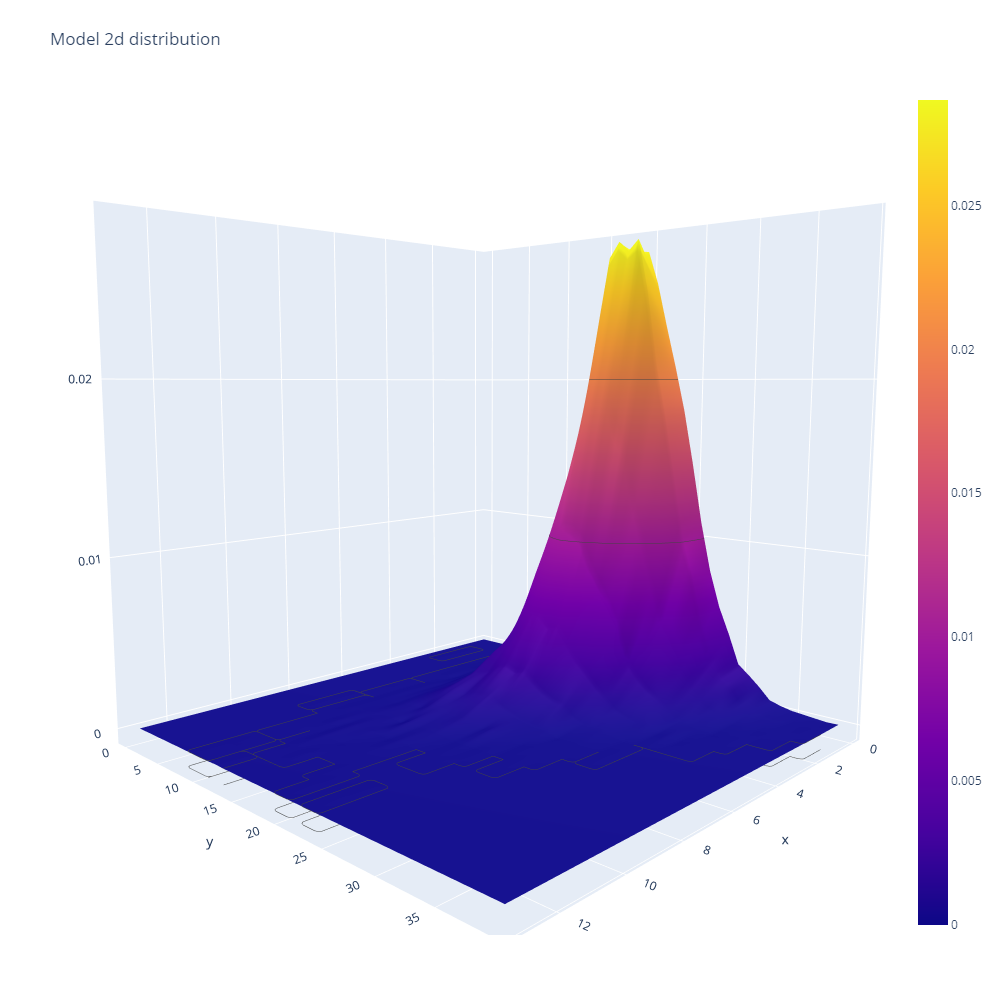
\includegraphics[scale=0.4]{model_2d_distr.png}
	\caption{Распределение числа обслуженных заявок по окончании имитационного моделирования} 
	\label{model_2d_distr}
\end{figure}

Теперь необходимо сравнить данное распределение вероятностей с аналогичным, но полученным при помощи асимптотического приближения характеристической функции числа обслуженных заявок. Для этого нам потребуется численно решить систему дифференциальных уравнений Колмогорова при помощи имеющегося в пакете класса RQSystem:

